%!TEX root = ../thesis.tex
% ******************************* Thesis Appendix D **********************************
\chapter[Δοκιμές επαλήθευσης]{Δοκιμές επαλήθευσης για τον προσδιορισμό σφαλμάτων}\label{app:actualitydata} 

% ******************************* Nomenclature ****************************************

\begin{table}[h!]
\centering
\sisetup{table-number-alignment = center, % <-- added/changed
         table-space-text-pre ={(},
         table-space-text-post={\textsuperscript{***}},
         input-open-uncertainty={[},
         input-close-uncertainty={]},
         table-align-text-pre=false,
         table-align-text-post=false}
\begin{threeparttable}
\caption{Δοκιμές επαλήθευσης χρονομέτρου και ψηφιακού πολυμέτρου}
\label{tab:rep1}
\begin{tabular}{@{}r 
                S[table-format=-2.3]
                 @{}}
\toprule
				   & {Παρτίδα μετρήσεων} \\
\cmidrule{2-2}		   
Μετρήσεις χρονομέτρου\\
$t$\tnote{*}       & 114.61\\
                   & (0.95)\\

Μετρήσεις πολυμέτρου\\
$V$\tnote{\dag}  	   & 29.48\\
                   & (0.11)\\
\addlinespace
$I$\tnote{\ddag}     & 0.63\\
                   & (0.01)\\
\midrule
Επαναλήψεις		   & 31\\
\bottomrule
\end{tabular}
    \smallskip
    \footnotesize
οι αριθμοί εκτός παρένθεσης είναι οι μέσες τιμές\par
οι αριθμοί εντός παρένθεσης είναι οι αντίστοιχες τυπικές αποκλίσεις\par
\begin{tablenotes}
\item[*]    μετρήσεις σε δευτερόλεπτα (\unit{\second})
\item[\dag]   μετρήσεις σε Volts (\unit{\volt})
\item[\ddag]  μετρήσεις σε Ampere (\unit{\ampere})
\end{tablenotes}
\end{threeparttable}
\end{table}


\begin{table}[h!]
\centering
\sisetup{table-number-alignment = center, % <-- added/changed
         table-space-text-pre ={(},
         table-space-text-post={\textsuperscript{***}},
         input-open-uncertainty={[},
         input-close-uncertainty={]},
         table-align-text-pre=false,
         table-align-text-post=false}
\begin{threeparttable}
\caption{Δοκιμές επαλήθευσης θερμοστοιχείων}
\label{tab:rep2}
\begin{tabular}{@{}l 
                S[table-format=-2.3]
                S[table-format=-2.3]
                S[table-format=-2.3]
                S[table-format=-2.3]
                S[table-format=-2.3]
                S[table-format=-2.3]
                @{}}
\toprule
                    & \multicolumn{6}{c}{Παρτίδες μετρήσεων} \\
\cmidrule(lr){2-7}
                    &   {(1)}           &   {(2)}           &  {(3)}  & {(4)} & {(5)}  &  {(6)}    \\
                    &	{\multirow[c]{2}*{αξονική}}	&	{$\alpha$\tnote{*} $= 1$}	&  {$\alpha = 2$}	&	{$\alpha = 3$}	&  {$\alpha = 4$} &	{$\alpha = 2$}	\\
                    &   & {$\phi$\tnote{**} $= \ang{45}$} & {$\phi = \ang{60}$} & {$\phi = \ang{75}$} & {$\phi = \ang{90}$} & {$\phi = \ang{90}$}	\\
                    &	{Re = 1420}		&	{Re\tnote{\dag} = 1826}		& {Re = 680} & {Re = 1200}	& {Re = 1640} & {Re = 640}\\
\midrule
$T_{\text{αντ, 1}}$& 30.36 & 28.92 & 31.76 & 29.61 & 28.66 & 27.88	\\
                    & (0.04) & (0.02) & (0.19) & (0.05) & (0.04) & (0.04)\\
\addlinespace
$T_{\text{αντ, 2}}$& 30.39 & 29.83 & 33.38 & 30.69 & 30.28 & 29.15	\\
                    & (0.04) & (0.02) & (0.48) & (0.05) & (0.03) & (0.04)\\
\addlinespace
$T_{\text{αντ, 3}}$& 30.67 & 30.93 & 34.78 & 32.03 & 31.93 & 30.49	\\
                    & (0.04) & (0.02) & (0.55) & (0.04) & (0.03) & (0.03)\\
\addlinespace
$T_{\text{αντ, 4}}$& 31.41 & 32.33 & 35.89 & 33.58 & 33.32 & 31.61	\\
                    & (0.04) & (0.01) & (0.55) & (0.03) & (0.03) & (0.03)\\
\addlinespace
$T_{\text{αντ, 5}}$& 31.69 & 33.25 & 36.18 & 34.66 & 33.74 & 31.87	\\
                    & (0.04) & (0.01) & (0.56) & (0.02) & (0.03) & (0.03)\\
\addlinespace
$T_{\text{αντ, 6}}$& 32.42 & 34.62 & 36.60 & 36.15 & 34.31 & 32.30	\\
                    & (0.03) & (0.02) & (0.55) & (0.01) & (0.03) & (0.03)\\
\addlinespace
$T_{\text{αντ, 7}}$& 31.13 & 35.77 & 36.77 & 37.39 & 34.64 & 32.56	\\
                    & (0.03) & (0.02) & (0.44) & (0.01) & (0.04) & (0.03)\\
\addlinespace
$T_{\text{αντ, 8}}$& 33.74 & 36.59 & 36.88 & 38.22 & 34.89 & 32.80	\\
                    & (0.03) & (0.02) & (0.31) & (0.02) & (0.04) & (0.03)\\
\addlinespace
$T_{\text{αντ, 9}}$& 34.06 & 37.02 & 36.67 & 38.71 & 35.34 & 33.27	\\
                    & (0.02) & (0.03) & (0.21) & (0.02) & (0.03) & (0.03)\\
\addlinespace
$T_{\text{εξ.}}$   & 34.37 & 41.10 & 32.75 & 37.30 & 30.73 & 31.64	\\
                   & (0.04) & (0.02) & (0.55) & (0.01) & (0.04) & (0.05)\\
\addlinespace
$T_{\infty}$       & 25.28 & 22.93 & 26.31 & 22.75 & 25.45 & 25.82	\\
                   & (0.02) & (0.01) & (0.01) & (0.01) & (0.02) & (0.08)\\
\midrule
Επαναλήψεις		   & 31 & 31 & 31 & 31 & 31 & 31 \\
\bottomrule
\end{tabular}
    \smallskip
    \footnotesize
οι αριθμοί εκτός παρένθεσης είναι οι μέσες τιμές, σε \unit{\degreeCelsius}\par
οι αριθμοί εντός παρένθεσης είναι οι αντίστοιχες τυπικές αποκλίσεις, σε \unit{\degreeCelsius}\par
\begin{tablenotes}[para,flushleft]
    \item[*]    αριθμός βρόγχων,
    \item[**]   γωνία βρόγχου,
    \item[\dag]  αριθμός Reynolds
    \end{tablenotes}
\end{threeparttable}
\end{table}



\begin{figure}[h!]
\centering
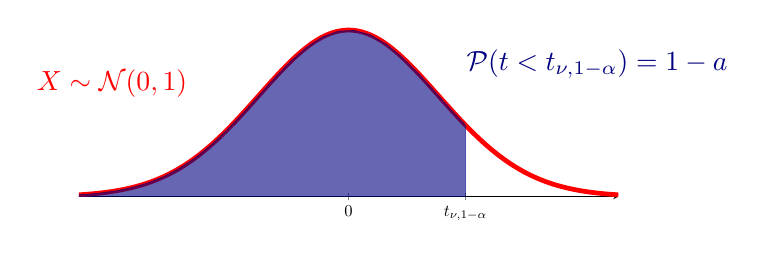
\begin{tikzpicture}[scale=0.6]

\def \xMoy{0};%moyenne

\def \ecartType {1};%ecart-type


\begin{axis}
[
axis x line=bottom,
axis y line=none,
xmin=-3,
xmax=3,
ymin=0,
ymax=0.5,
xtick={0,1.3},
xticklabels={0,$t_{\scriptstyle{\nu,1-\alpha}}$},
enlarge x limits=-1, %hack to plot on the full x-axis scale
width=13cm, %set bigger width
height=6cm,
]

\addplot+[mark=none,domain=-3:3,samples=200,color=red,smooth,line width=1mm]{(exp(-(x-\xMoy)^2/(2*\ecartType^2)))/(\ecartType*sqrt(6.28))}; 


\addplot+[mark=none,fill=NavyBlue,draw=NavyBlue,opacity=0.6,domain=-25:1.3,samples=150]{(exp(-(x-\xMoy)^2/(2*\ecartType^2)))/(\ecartType*sqrt(6.28))}\closedcycle;

\end{axis}
%\Phi(a)=P(X\le a)$
\draw (8,2.8) node[right] { {\color{NavyBlue} $\mathcal{P}(t < t_{\scriptstyle{\nu,1-\alpha}}) = 1 - a$}};
\draw (2.5,2.4) node[left] { {\color{red} $X  \sim \mathcal{N}(0,1)$}};

\end{tikzpicture}
\end{figure}

\begin{table}[h!]
\centering
\sisetup{table-number-alignment = center, % <-- added/changed
         table-space-text-pre ={(},
         table-space-text-post={\textsuperscript{***}},
         input-open-uncertainty={[},
         input-close-uncertainty={]},
         table-align-text-pre=false,
         table-align-text-post=false}
\begin{adjustbox}{width=\textwidth}
\begin{threeparttable}
\caption{Στατιστικός Πίνακας Κατανομής Student}
\label{tab:student}
\begin{tabular}{@{}l 
                S[table-format=-2.3]
                S[table-format=-2.3]
                S[table-format=-2.3]
                S[table-format=-2.3]
                S[table-format=-2.3]
                S[table-format=-2.3]
                S[table-format=-2.3]
                S[table-format=-2.3]
                S[table-format=-2.3]
                S[table-format=-2.3]
                S[table-format=-2.3]
                 @{}}
\toprule
& \multicolumn{11}{c}{$1 - \alpha$\tnote{**}}\\
\cmidrule{2-12}
$\nu$\tnote{*}&60.0\% & 66.7\%&75.0\%&80.0\%&87.5\%&90.0\%&95.0\%& \color{NavyBlue} 97.5\% &99.0\%&99.5\% &99.9\% \\
\midrule
 1&0.325&0.577&1.000&1.376&2.414&3.078&6.314&12.706&31.821&63.657&318.31 \\
 2&0.289&0.500&0.816&1.061&1.604&1.886&2.920&4.303&6.965&9.925&22.327 \\
 3&0.277&0.476&0.765&0.978&1.423&1.638&2.353&3.182&4.541&5.841&10.215 \\
 4&0.271&0.464&0.741&0.941&1.344&1.533&2.132&2.776&3.747&4.604&7.173 \\
\color{NavyBlue} 5&0.267&0.457&0.727&0.920&1.301&1.476&2.015&\color{red} 2.571&3.365&4.032&5.893 \\
 \addlinespace
 6&0.265&0.453&0.718&0.906&1.273&1.440&1.943&2.447&3.143&3.707&5.208 \\
 7&0.263&0.449&0.711&0.896&1.254&1.415&1.895&2.365&2.998&3.499&4.785 \\
 8&0.262&0.447&0.706&0.889&1.240&1.397&1.860&2.306&2.896&3.355&4.501 \\
 9&0.261&0.445&0.703&0.883&1.230&1.383&1.833&2.262&2.821&3.250&4.297 \\
10&0.260&0.444&0.700&0.879&1.221&1.372&1.812&2.228&2.764&3.169&4.144 \\
\addlinespace
11&0.260&0.443&0.697&0.876&1.214&1.363&1.796&2.201&2.718&3.106&4.025 \\
12&0.259&0.442&0.695&0.873&1.209&1.356&1.782&2.179&2.681&3.055&3.930 \\
13&0.259&0.441&0.694&0.870&1.204&1.350&1.771&2.160&2.650&3.012&3.852 \\
14&0.258&0.440&0.692&0.868&1.200&1.345&1.761&2.145&2.624&2.977&3.787 \\
15&0.258&0.439&0.691&0.866&1.197&1.341&1.753&2.131&2.602&2.947&3.733 \\
\addlinespace
16&0.258&0.439&0.690&0.865&1.194&1.337&1.746&2.120&2.583&2.921&3.686 \\
17&0.257&0.438&0.689&0.863&1.191&1.333&1.740&2.110&2.567&2.898&3.646 \\
18&0.257&0.438&0.688&0.862&1.189&1.330&1.734&2.101&2.552&2.878&3.610 \\
19&0.257&0.438&0.688&0.861&1.187&1.328&1.729&2.093&2.539&2.861&3.579 \\
20&0.257&0.437&0.687&0.860&1.185&1.325&1.725&2.086&2.528&2.845&3.552 \\
\addlinespace
21&0.257&0.437&0.686&0.859&1.183&1.323&1.721&2.080&2.518&2.831&3.527 \\
22&0.256&0.437&0.686&0.858&1.182&1.321&1.717&2.074&2.508&2.819&3.505 \\
23&0.256&0.436&0.685&0.858&1.180&1.319&1.714&2.069&2.500&2.807&3.485 \\
24&0.256&0.436&0.685&0.857&1.179&1.318&1.711&2.064&2.492&2.797&3.467 \\
25&0.256&0.436&0.684&0.856&1.178&1.316&1.708&2.060&2.485&2.787&3.450 \\
\addlinespace
26&0.256&0.436&0.684&0.856&1.177&1.315&1.706&2.056&2.479&2.779&3.435 \\
27&0.256&0.435&0.684&0.855&1.176&1.314&1.703&2.052&2.473&2.771&3.421 \\
28&0.256&0.435&0.683&0.855&1.175&1.313&1.701&2.048&2.467&2.763&3.408 \\
29&0.256&0.435&0.683&0.854&1.174&1.311&1.699&2.045&2.462&2.756&3.396 \\
\color{NavyBlue} 30&0.256&0.435&0.683&0.854&1.173&1.310&1.697& \color{red} 2.042 &2.457&2.750&3.385 \\
\addlinespace
35&0.255&0.434&0.682&0.852&1.170&1.306&1.690&2.030&2.438&2.724&3.340 \\
40&0.255&0.434&0.681&0.851&1.167&1.303&1.684&2.021&2.423&2.704&3.307 \\
45&0.255&0.434&0.680&0.850&1.165&1.301&1.679&2.014&2.412&2.690&3.281 \\
50&0.255&0.433&0.679&0.849&1.164&1.299&1.676&2.009&2.403&2.678&3.261 \\
55&0.255&0.433&0.679&0.848&1.163&1.297&1.673&2.004&2.396&2.668&3.245 \\
60&0.254&0.433&0.679&0.848&1.162&1.296&1.671&2.000&2.390&2.660&3.232 \\
$\infty$ &0.253&0.431&0.674&0.842&1.150&1.282&1.645&1.960&2.326&2.576&3.090\\
\bottomrule
\end{tabular}
    \smallskip
    \footnotesize
ο πίνακας δημιουργήθηκε βάσει \url{https://www.york.ac.uk/depts/maths/tables/t.htm}
\begin{tablenotes}[para,flushleft]
    \item[*] βαθμοί ελευθερίας,
    \item[**] τιμή της αθροιστικής συνάρτησης
    \end{tablenotes}\par
οι {\color{red} κοκκινισμένοι} συντελεστές διόρθωσης χρησιμοποιήθηκαν στην παρούσα εργασία
\end{threeparttable}
\end{adjustbox}
\end{table}